%This template (2022-02-06) is a modified version by Magnus Andersson (Department of physics) and TF student Jesper Erixon of the Stylish Article LaTeX Template Version 2.1 (1/10/15)
% Original author:
% Mathias Legrand (legrand.mathias@gmail.com) 
%
% License:
% CC BY-NC-SA 3.0

%----------------------------
\documentclass[fleqn,10pt]{SelfArx} % Document font size and equations flushed left
\usepackage[english]{babel} % Specify a different language here - English by default
\usepackage{lipsum} % Required to insert dummy text. To be removed otherwise
\usepackage{float} % Allow you to set the figure at a specific position, use mainly H
% Additional packages
\usepackage{subcaption} % Allow you to create subfigures with individual captions
\usepackage{amsmath}
\usepackage{esvect}
\usepackage{caption}
\usepackage{caption}
\usepackage{subcaption}
\captionsetup[figure]{font=small}
\usepackage[font=small,labelfont=bf,justification=justified]{caption}
\usepackage[font=small,labelfont=bf,justification=justified]{subcaption}
%\usepackage{acro}

%\DeclareAcronym{usa}{
%  short=USA,
%  long=United States of America,
%}
\usepackage{hyperref}
%----------------------------
%	COLUMNS
%----------------------------
\setlength{\columnsep}{0.55cm} % Distance between the two columns of text
\setlength{\fboxrule}{0.75pt} % Width of the border around the abstract
%----------------------------
%	COLORS
%----------------------------
\definecolor{color1}{RGB}{0,0,90} % Color of the article title and sections
\definecolor{color2}{RGB}{0,20,20} % Color of the boxes behind the abstract and headings
%----------------------------
%	HYPERLINKS
%----------------------------
\usepackage{hyperref} % Required for hyperlinks
\hypersetup{hidelinks, colorlinks,colorlinks=true,breaklinks=true,urlcolor=color1,citecolor=color1,linkcolor=color1,bookmarksopen=false,pdftitle={Title},pdfauthor={Author}}
% \hypersetup{
%     colorlinks=true,
%     linkcolor=color1,
%     urlcolor=color1,
%     citecolor=color1
%}
\urlstyle{same} % Sets url font
\usepackage{cleveref} % Added: Use cleveref to be able to reference subfigures e.g. Fig 1(a) etc.
\captionsetup[subfigure]{subrefformat=simple,labelformat=simple} % Added: Setup subfigure label
\renewcommand\thesubfigure{(\alph{subfigure})}
%----------------------------
%	ARTICLE INFORMATION
%----------------------------
\JournalInfo{Deep Learning - methods and applications}
\Archive{\today}

%\PaperTitle{Optimering av lagerhantering samt utveckling av ett simuleringsverktyg för Cytiva} % Article title

%\Authors{Alma Wikström, Christine Sandström, Ellinor Olsson, Emmeline Kjellgren, Sovann Mong, Theodor Jonsson} % Authors
\affiliation{\textsuperscript{1}\textit{Department of Physics, Umeå University, Umeå, Sweden}} % Author affiliation
\affiliation{*\textbf{Corresponding author}: thjo0148@student.umu.se, sose0037@student.umu.se, elol1002@student.umu.se, chsa0129@student.umu.se, emkj0013@student.umu.se, alwi0072@student.umu.se} % Corresponding author
\affiliation{\textbf{Supervisor}: martin.rosvall@umu.se\textsuperscript{1}}
\Keywords{Simulering, lagerhantering, Min-Max strategi} % Keywords - if you don't want any simply remove all the text between the curly brackets
\newcommand{\keywordname}{Keywords} % Defines the keywords heading name
\usepackage[printonlyused,withpage]{acronym}
\begin{document}

%----------------------------
%	TITLE PAGE
%----------------------------
\begin{titlepage}
\begin{center}
        \vspace*{1cm}
            
        \Huge
        \textbf{Image segmentation of brain cancer tumors using a U-Net architecture with residual connections.}
            
        \vspace{0.5cm}
        \LARGE
        \href{https://www.umu.se/utbildning/kursplan/5tf078/rev/32737/}{Deep Learning - methods and applications (5TF078)}

            
        \vspace{1.5cm}
        \large
            
        \textbf{Author}
       
        Theodor Jonsson  thjo0148@student.umu.se\\

       
    

        
         %\textbf{Xiaoying Zhang}
         
        %\textcolor{red}{Who dis?}
        
        \vfill

       
            
            
        \vspace{0.8cm}
            
        
\includegraphics[width=0.4\textwidth]{university}
        
          
        \Large
        Department of Applied Physics and Electronics\\
        Umeå University\\
        Sweden\\
        \today
            
    \end{center}
    
\end{titlepage}

%----------------------------

%----------------------------
%	ABSTRACT
%----------------------------
\Abstract{
This study focuses on the optimization of the inventory management for Cytiva's department located in Umeå. Cytiva is a global company operating in the life science industry. The aim is to develop a simulation tool that can analyze and optimize Cytiva's inventory by examining parameters such as lead time and quantity. The tool will provide insights into the future turns and inventory value of the warehouse based on changes in these parameters. Additionally, it will offer recommendations for the implementation of the Min-Max strategy on specific articles, enhancing inventory efficiency. The research methodology includes data analysis, simulation, and usability considerations. The simulation tool is designed to be user-friendly, providing an intuitive graphical user interface (GUI) for easy interaction and validation of Min-Max parameters. The results of the project include the development of the simulation tool and its application to Cytiva's inventory, contributing to more efficient inventory management and optimization strategies.
}

%----------------------------


\flushbottom % Makes all text pages the same height

\maketitle % Print the title and abstract box
\tableofcontents % Print the contents section

\thispagestyle{empty} % Removes page numbering from the first page

%----------------------------
%	ARTICLE CONTENTS
%----------------------------

%----------------------------
%\section*{Acronyms}
%\printacronyms

\section{Introduction}
% Inledningen bör innehålla:
% Problemformulering
% Bakgrund till problemet
% Mål, syfte och eventuella avgränsningar
% Motivation till valda metod och arbetssätt
% Rapportens disposition och eventuella råd till läsaren
The task of segmenting images has been an important task within computer vision for several years. During this time it has been used in a variety of applications including; video editing, robotics, autonomous driving, and many more. This paper focuses on applying image segmentation to segment cancerous tumors in the brain from CT scans. This technology has been used to assist radiologists in many hospitals across the world. Specifically, this paper discusses the use of a U-Net \cite{Unet} with a ResNet-like structure \cite{ResNet}. The models used in this paper were trained on a subset of the of the \href{https://www.kaggle.com/datasets/awsaf49/brats2020-training-data?resource=download}{BraTs 2019} dataset and were supplied via the course \href{https://www.umu.se/en/education/courses/convolutional-neural-networks-with-applications-in-medical-image-analysis/}{Convolutional Neural Networks with Applications in Medical Image Analysis} and can be found in the \href{https://github.com/Tottowich/AppliedDL-project}{Github repository} containing the code of this project.
\\\\\noindent
Using deep learning in the medical domain means that we must be able to explain the results of the model. If we can't measure any form of uncertainty in the model's predictions then we can't say if the prediction is a result of some statistical anomaly. Therefore this paper also discusses the uncertainty in the model using Monte Carlo dropout for uncertainty estimation to further improve the robustness of the model's predictions suitable in for medical applications.
\section{Theory}
\subsection{Evaluation - Dice score}
To construct and train a model we must find a way to evaluate a model on a segmentation task. One common way to evaluate the model is to use the Sørensen–Dice coefficient or more commonly referred to as the \emph{Dice score}. This measures the amount of overlap per class and divides it by the total number of classes or mathematically:
\begin{equation}
\label{eq:DiceScore}
    D = \frac{2\left|\hat{Y}\cap Y\right|}{\left|\hat{Y}\right|+\left|Y\right|}.
\end{equation}
Where $\hat{Y}$ is the model's prediction per pixel and $Y$ is the ground truth label. This metric has been used to determine the model's capability to segment the binary masks correctly.\cite{Dice} To train the model we can then construct the Dice loss.
\subsection{Loss function - Focal dice loss}
The dice loss is used to optimize the dice score via 
\begin{equation}
\label{eq:DiceLoss}
    \ell_D = 1 - D
\end{equation}
where $D$ is the dice score as described in Eq. \ref{eq:DiceScore}. This loss would optimize for the dice score but due to imbalances in the class distributions, this would probably result in only predictions of the background. Instead, we utilize a combination between Focal loss and dice loss. Focal loss is a way to penalize the prediction of the more common background class by adding a regularizing to the loss function in the form of
\begin{equation}
\label{eq:Focal}
    \ell_{F} = -\alpha\left((1-Y)\cdot(1-\hat{Y})^\gamma\log\left(1-\hat{Y}\right)+Y\cdot\hat{Y}^\gamma\log\hat{Y}\right).
\end{equation}
Notice that if $\gamma=0 \text{ and } \alpha=1$ then this would be the usual binary cross entropy loss.\cite{Focal} The loss function during training was then:
\begin{equation}
    \label{eq:loss}
    \ell = w_F\cdot\ell_F + w_D\cdot\ell_D
\end{equation}
Where $w_F$ and $w_D$ are relative importance hyper-parameters.
\section{Method}
The main parts of training and evaluating a deep learning model is to 
\begin{enumerate}
  \setlength{\itemsep}{5pt}
  \setlength{\parskip}{5pt}
    \item Find an appropriate dataset.
    \item Process the data such that it can be interpreted by the model.
    \item Determine the hypothesis space and the loss function which together construct the model.
    \item Train the model.
    \item Evaluate the model.
\end{enumerate}
\subsection{BraTS}
The BraTS dataset is a dataset containing \textbf{Bra}in \textbf{T}umor \\\textbf{S}egmentations hence the abbreviation \textbf{BraTS}. The dataset is part of an annual challenge designed to improve the segmentation models used in radiology today.\cite{brats}

The specific version used during this project is available through the project's \href{https://github.com/Tottowich/AppliedDL-project}{Github} in the form of NumPy slices of the 3D scans. The scans consist of 4 different scanning formats.
\begin{itemize}
  \setlength{\itemsep}{5pt}
  \setlength{\parskip}{5pt}
    \item T1-weighted visualizes the various tissues in the scan. Higher value implies higher fat content.
    \item T2-weighted visualizes the differences in water content per tissue. Fluids appear brighter than solids such as bone or such.
    \item FLAIR or Fluid-Attenuated Inversion Recovery suppresses the liquid material making it easier to see abnormalities in the scans.
    \item T1CE are T1-weighted images with increased contrast (Contrast-enhanced).\cite{mri}
\end{itemize}
\subsubsection{Pre-processing}
In order to make the inputs more model friendly we utilized pre-processing in the form of normalizing and zooming, i.e. centering the image and removing redundant background. We also utilize all possible information about the image by stacking the images as a 4-dimensional image, one per scan format. In summary, the initial $(256\times256)$ image that are available per format is stacked, normalized and cropped to create a $(64\times64\times4)$ input. 
\subsection{Model Architecture}
The model architecture can be seen in the Appendix figure \ref{fig:arch} and is a modification of the typical U-Net, see figure \ref{fig:unet}. These modifications are:
\begin{itemize}
  \setlength{\itemsep}{0pt}
  \setlength{\parskip}{0pt}
    \item Internal residual connections similar to a ResNet architecture.
    \item A deeper and larger network with larger minimum latent space representation.
\end{itemize}
\begin{figure}[h]
    \centering
    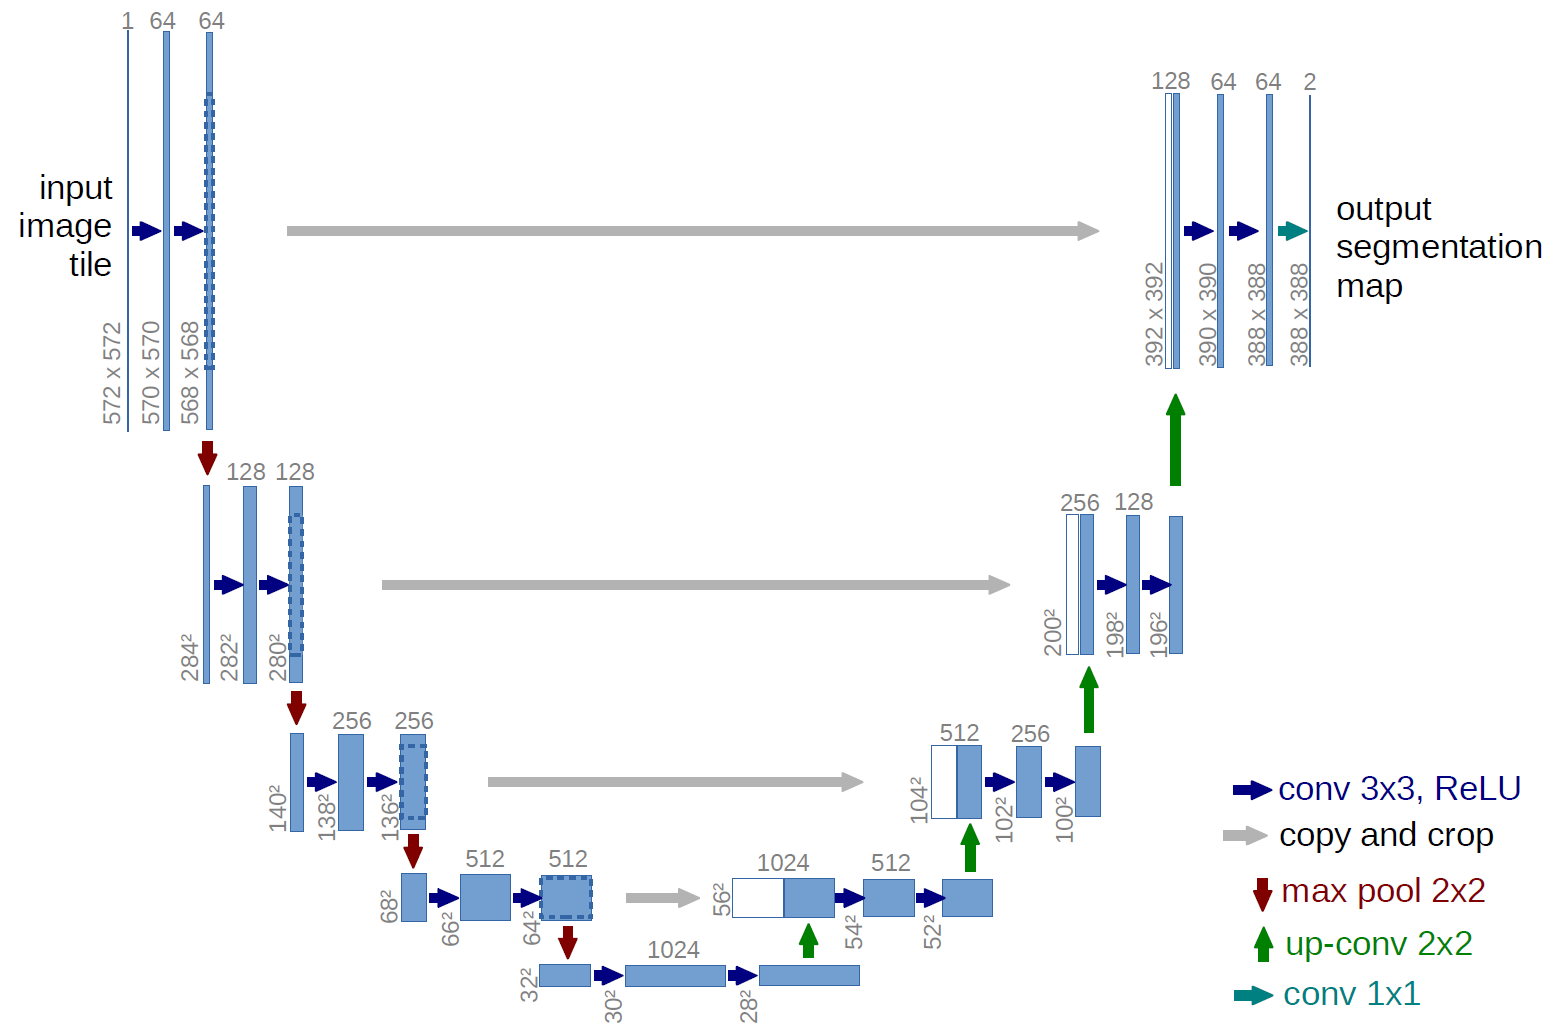
\includegraphics[width=\linewidth]{report/Images/u-net-architecture.png}
    \caption{The original U-Net architecture. It is clearly visualized how the skip connections are used as context in the decoder to produce a valid segmentation map.\cite{Unet}}
    \label{fig:unet}
\end{figure}
\subsubsection{Residual Blocks}
The "residual\_block" is one of the main additions to the base U-Net model. It is a typical ResNet block and has the following structure:
\begin{figure}[H]
    \centering
    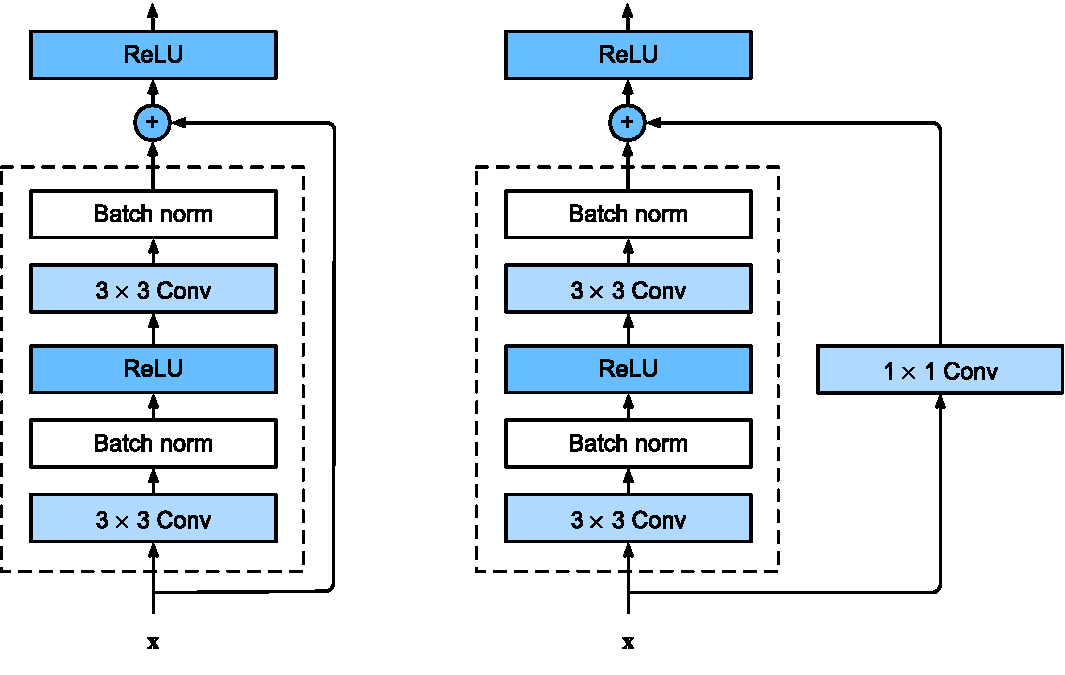
\includegraphics[width=\linewidth]{report/Images/resnet-block.pdf}
    \caption{Visualization of the "residual\_block". To the right is the structure of the residual block if it is the first in its depth cycle. To the left is all consecutive blocks after the initial residual block per depth.}
    \label{fig:res_block}
\end{figure}
The image above demonstrates how the internal skip-connections are constructed. After every down- or up-sampling layer there is a depth of residual blocks. The image demonstrates the two possibilities of how the blocks are constructed, one if it is the initial block at the current depth (left) and the other (right) if it is one of the later blocks per depth.
\subsubsection{Encoder}
The structure of the encoder was $5$ layers with residual blocks 1 residual block per layer. To reduce the dimensionality of the activation maps produced there was a max pooling layer to reduce the height and width per activation map by half in between each layer of the residual block.

\begin{table}[!h]
  \centering
  \caption{Encoder architecture. Each layer produces one output which is used as context in the decoder. The internal depth represents the number of residual blocks.}
  \label{tab:model_architecture}
  \begin{tabular}{|c|c|c|}
    \hline
    \textbf{Layer} & \textbf{Output Shape} & \textbf{Internal depth}\\
    \hline
    \hline
    Input & ($64\times64\times4$) & $1$\\
    \hline
    $1$ & ($32\times32\times16$) & $1$\\
    \hline
    $2$ & ($16\times16\times32$) & $1$\\
    \hline
    $3$ & ($8\times8\times64$) & $1$\\
    \hline
    $4$ & ($4\times4\times128$) & $1$\\
    \hline
    $5$ & ($2\times2\times128$) & $1$\\
    \hline
  \end{tabular}
\end{table}
\subsubsection{Decoder}
The decoder has the task to reconstruct an image from the feature maps produced by the encoder. In a U-Net architecture, the decoder uses the intermediate feature maps through concatenation with the features which has been passed through the entire network, see figure \ref{fig:unet} for reference. The decoder uses the results of the encoder to produce a segmentation map which is then
\begin{table}[!h]
  \centering
  \caption{Decoder architecture. Each layer produces one output which is used as context in the decoder. The internal depth represents the number of residual blocks.}
  \label{tab:model_architecture}
  \begin{tabular}{|c|c|c|}
    \hline
    \textbf{Layer} & \textbf{Output Shape} & \textbf{Internal depth}\\
    \hline
    \hline
    Input & ($2\times2\times256$) & $1$\\
    \hline
    $1$ & ($4\times4\times256$) & $1$\\
    \hline
    $2$ & ($8\times8\times128$) & $1$\\
    \hline
    $3$ & ($16\times16\times64$) & $1$\\
    \hline
    $4$ & ($32\times32\times32$) & $1$\\
    \hline
    $5$ & ($64\times64\times16$) & $1$\\
    \hline
    Output block & ( $64\times64\times1$) & $1$\\
    \hline
  \end{tabular}
\end{table}
\subsection{Training Process}
The training process consisted of three parts; data augmentation, model optimization, and hold-off validation.
\subsubsection{Data Augmentation}
To reduce overfitting and make the model generalize better we added data augmentation as a step in the pre-processing. The augmentation contained
\begin{itemize}
    \item Flipping the image in both x and y direction.
    \item Masking parts of the input image.
    \item Adding noise to the input image.
\end{itemize}
To see the results of the augmentation you can see some input samples in appendix, figure \ref{fig:train_inputs}. 
%------------------------------------------------
\section{Results}
% \begin{figure}[h]
%     \centering
%     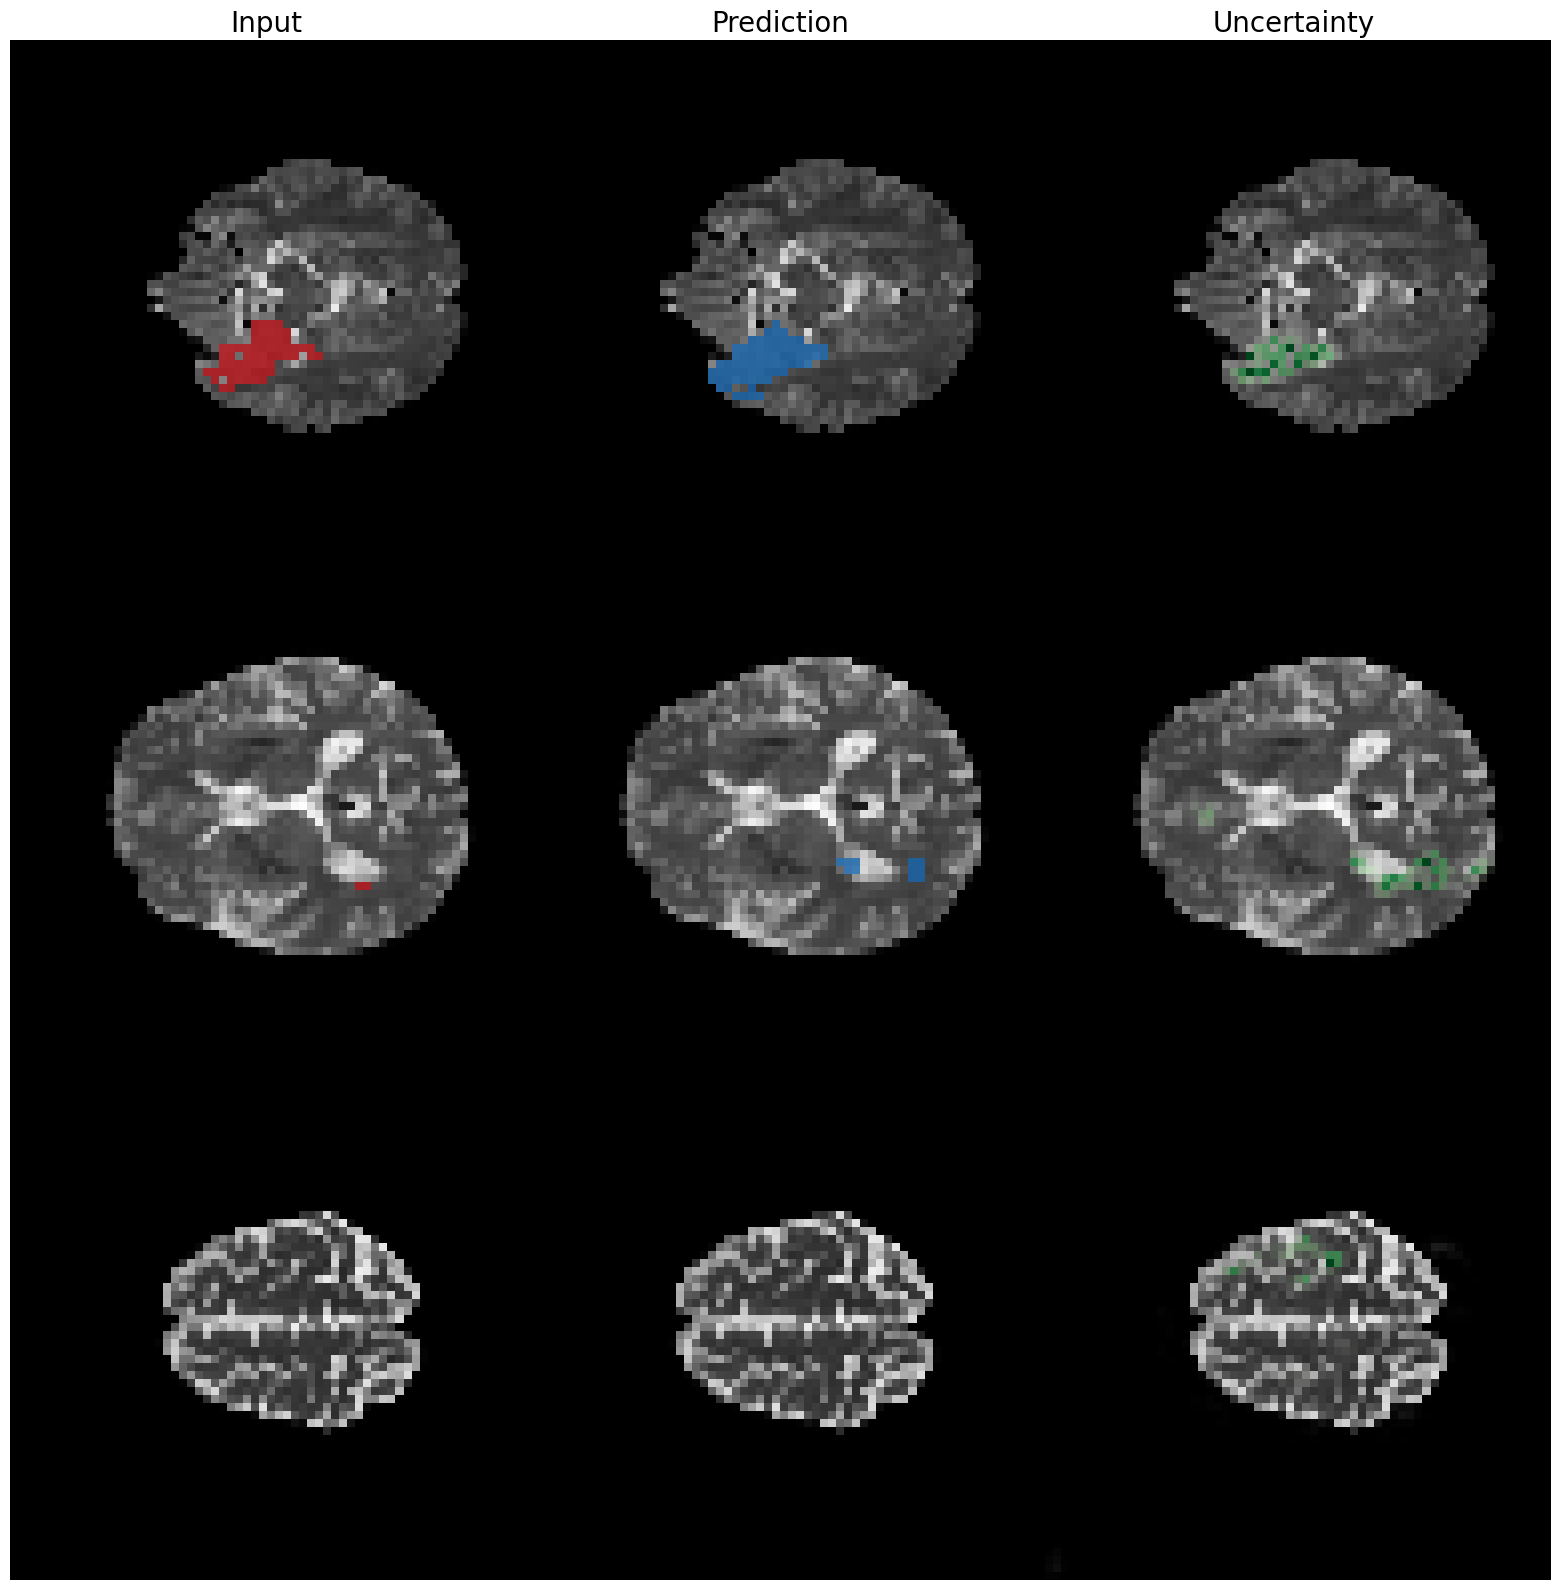
\includegraphics[width=0.95\linewidth]{report/Images/test_set.png}
%     \caption{Grafiskt användargränsnitt framställt för att enkelt utföra simuleringen.}
%     \label{fig:gui}
% \end{figure}

\section{Discussion}
% Kritisk granskning och diskussion av resultat.
% Utredning om syftet uppnåtts samt vilka möjligheter till vidareutveckling det finns 


%----------------------------
%	REFERENCE LIST
%----------------------------
\bibliographystyle{model1-num-names}
\begin{thebibliography}{2}
    
\bibitem{Unet}
    Arxiv. \emph{U-Net: Convolutional Networks for Biomedical Image Segmentation}. 2015.
    Olaf Ronneberger, Philipp Fischer, Thomas Brox.
    \url{https://arxiv.org/abs/1505.04597} (Retrieved 2023-06-3)
\bibitem{ResNet}
    Arxiv. \emph{Deep Residual Learning for Image Recognition}. 2015.
    Kaiming He, Xiangyu Zhang, Shaoqing Ren, Jian Sun.
    \url{https://arxiv.org/abs/1512.03385} (Retrieved 2023-06-3)
\bibitem{Dice}
    Wikipedia. \emph{Sørensen-Dice coefficient}. Available online: \url{https://en.wikipedia.org/wiki/S\%C3\%B8rensen\%E2\%80\%93Dice_coefficient} (Retrieved 2023-06-04).
\bibitem{Focal}
    Tsung-Yi Lin Priya Goyal Ross Girshick Kaiming He Piotr Dollar´
    Facebook AI Research (FAIR). \emph{Focal Loss for Dense Object Detection}. 2017. Available online: \url{https://arxiv.org/pdf/1708.02002.pdf} (Retrieved 2023-06-04).
\bibitem{brats}
    Menze BH, Jakab A, Bauer S, Kalpathy-Cramer J, Farahani K, Kirby J, Burren Y, Porz N, Slotboom J, Wiest R, Lanczi L, Gerstner E, Weber MA, Arbel T, Avants BB, Ayache N, Buendia P, Collins DL, Cordier N, Corso JJ, Criminisi A, Das T, Delingette H, Demiralp Ç, Durst CR, Dojat M, Doyle S, Festa J, Forbes F, Geremia E, Glocker B, Golland P, Guo X, Hamamci A, Iftekharuddin KM, Jena R, John NM, Konukoglu E, Lashkari D, Mariz JA, Meier R, Pereira S, Precup D, Price SJ, Raviv TR, Reza SM, Ryan M, Sarikaya D, Schwartz L, Shin HC, Shotton J, Silva CA, Sousa N, Subbanna NK, Szekely G, Taylor TJ, Thomas OM, Tustison NJ, Unal G, Vasseur F, Wintermark M, Ye DH, Zhao L, Zhao B, Zikic D, Prastawa M, Reyes M, Van Leemput K. The Multimodal Brain Tumor Image Segmentation Benchmark (BRATS). IEEE Trans Med Imaging. 2015 Oct;34(10):1993-2024. doi: 10.1109/TMI.2014.2377694. Epub 2014 Dec 4. PMID: 25494501; PMCID: PMC4833122.
\bibitem{mri}
https://case.edu/med/neurology/NR/MRI%20Basics.htm
    Case Western Reserve. \emph{Magnetic Resonance Imaging (MRI) of the Brain and Spine: Basics}. Available online: \url{https://case.edu/med/neurology/NR/MRI\%20Basics.htm} (Retrieved 2023-06-04).
\end{thebibliography}


%-----------------------------------------------
\phantomsection %Remove this section when you save your PDF
\setcounter{figure}{0}\renewcommand\thefigure{A\arabic{figure}}\renewcommand\thetable{A\arabic{table}}
\label{Appendix}
\begin{figure*}[!t]
    \centering
    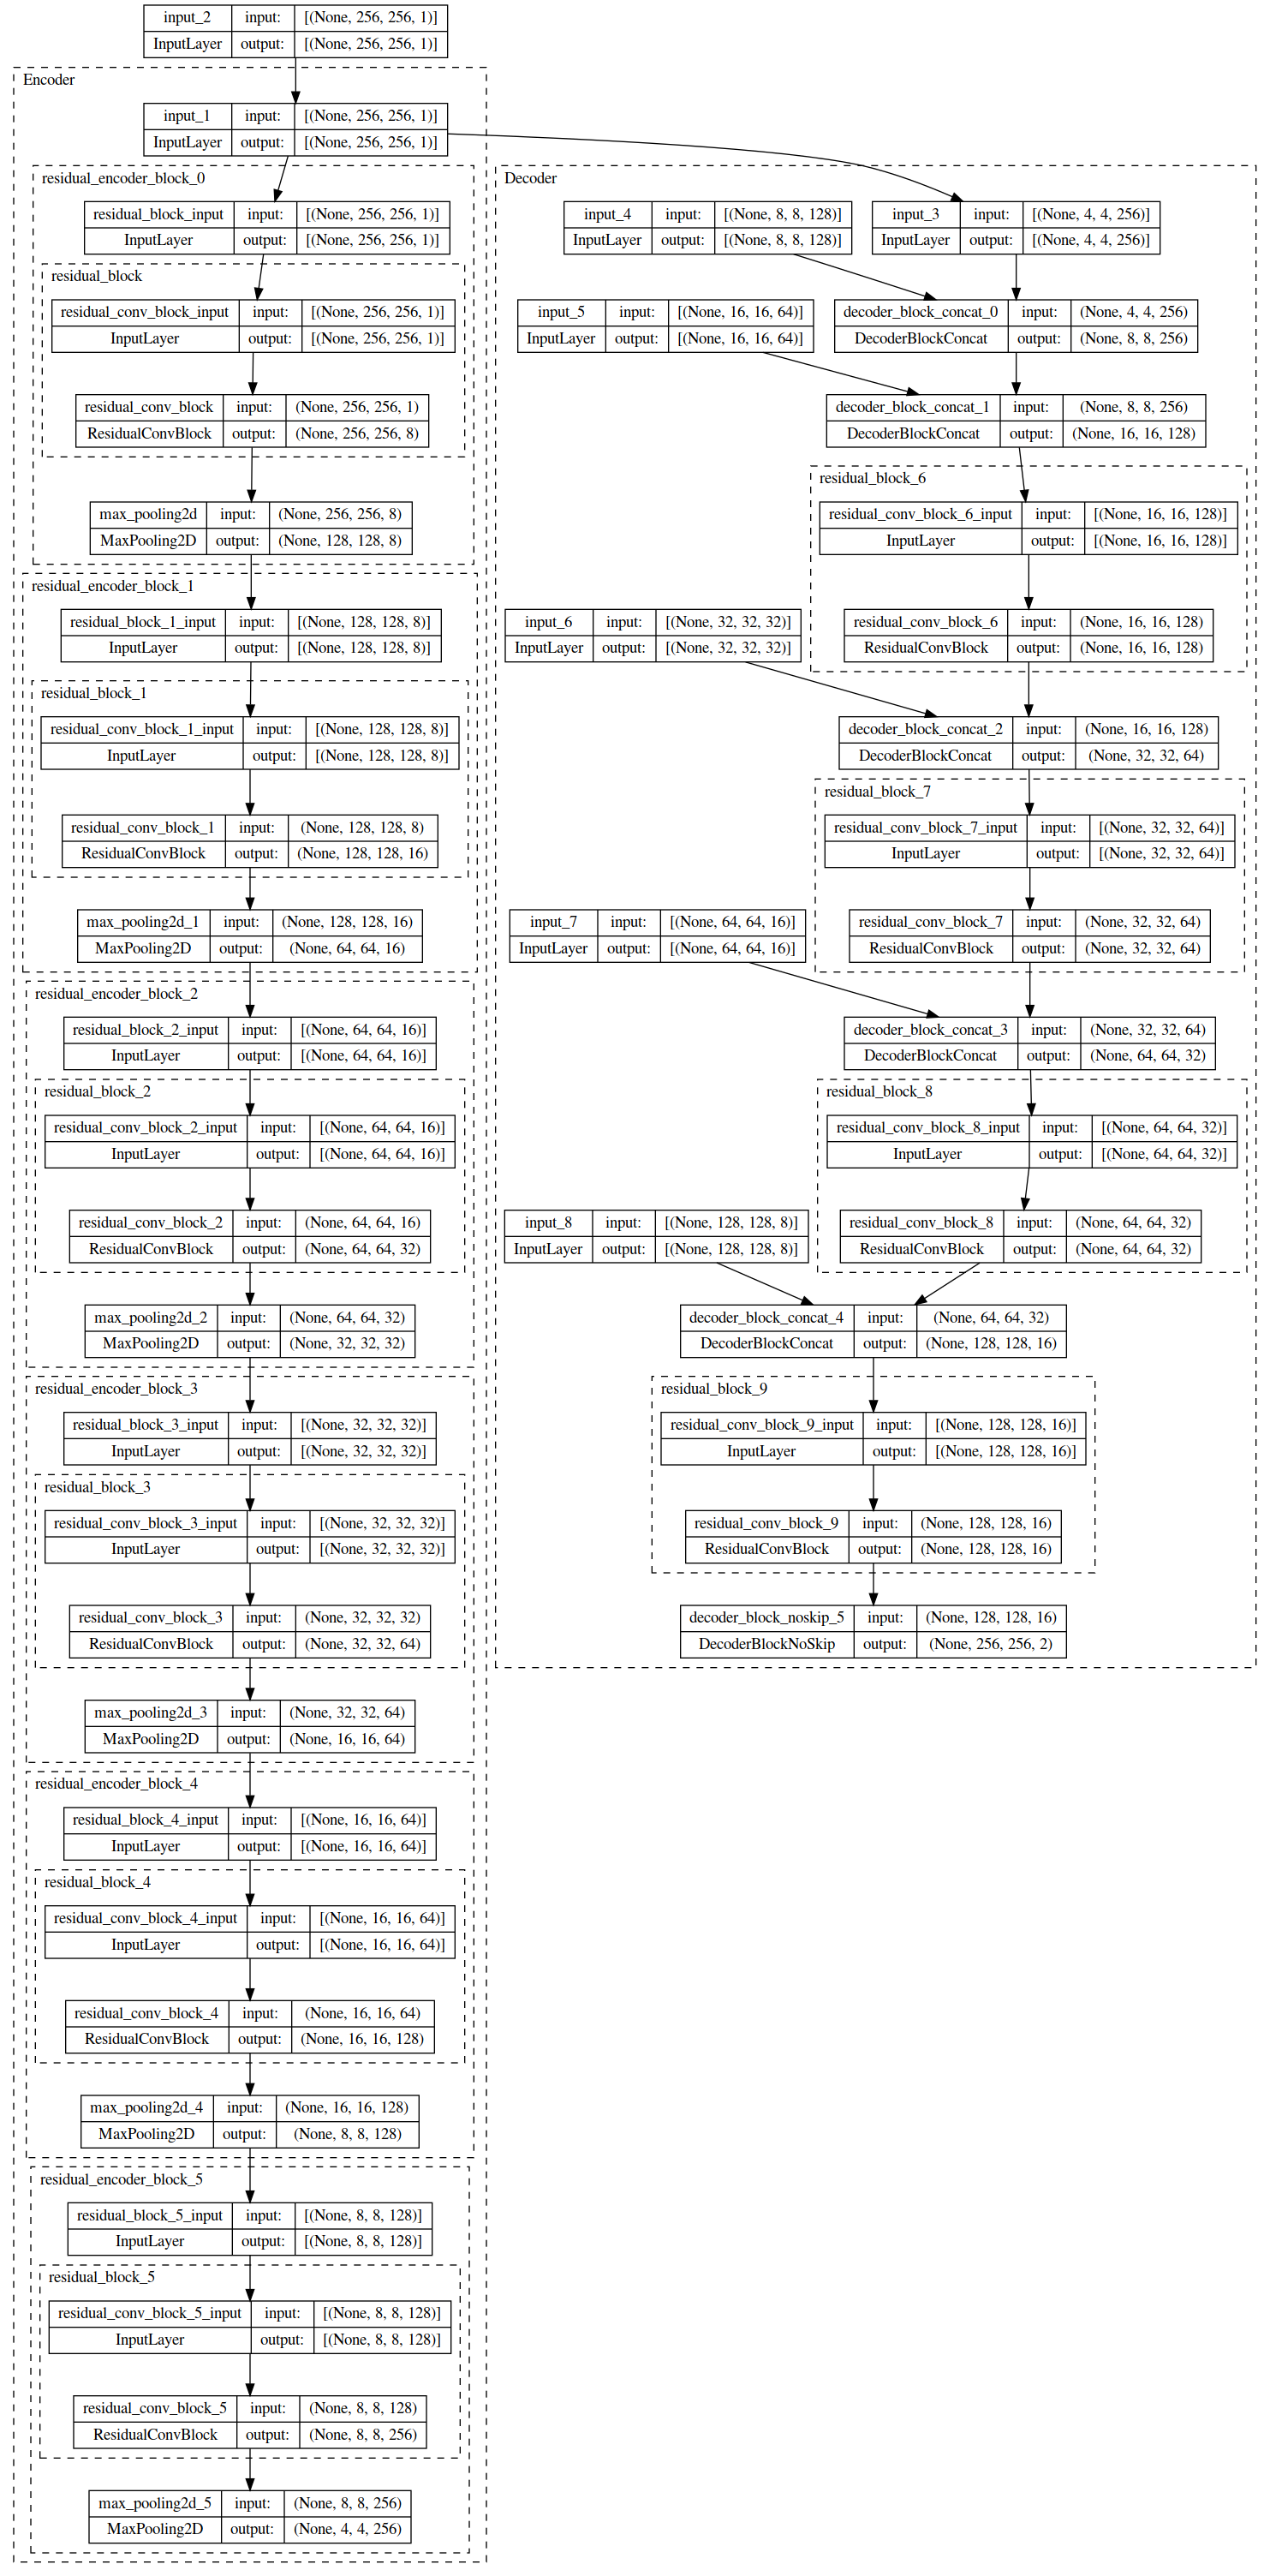
\includegraphics[width=0.9\textwidth]{report/Images/unet.png}
    \caption{The U-Net model architecture with residual connection blocks. These blocks are regular ResNet blocks consisting of convolutions, activations, batch normalizations, and a highway skip connection. The used activation function was the standard ReLU function. This model had a total of $2,255,121$ trainable parameters.}
    \label{fig:arch}
\end{figure*}
\newpage
\begin{figure*}[!t]
    \centering
    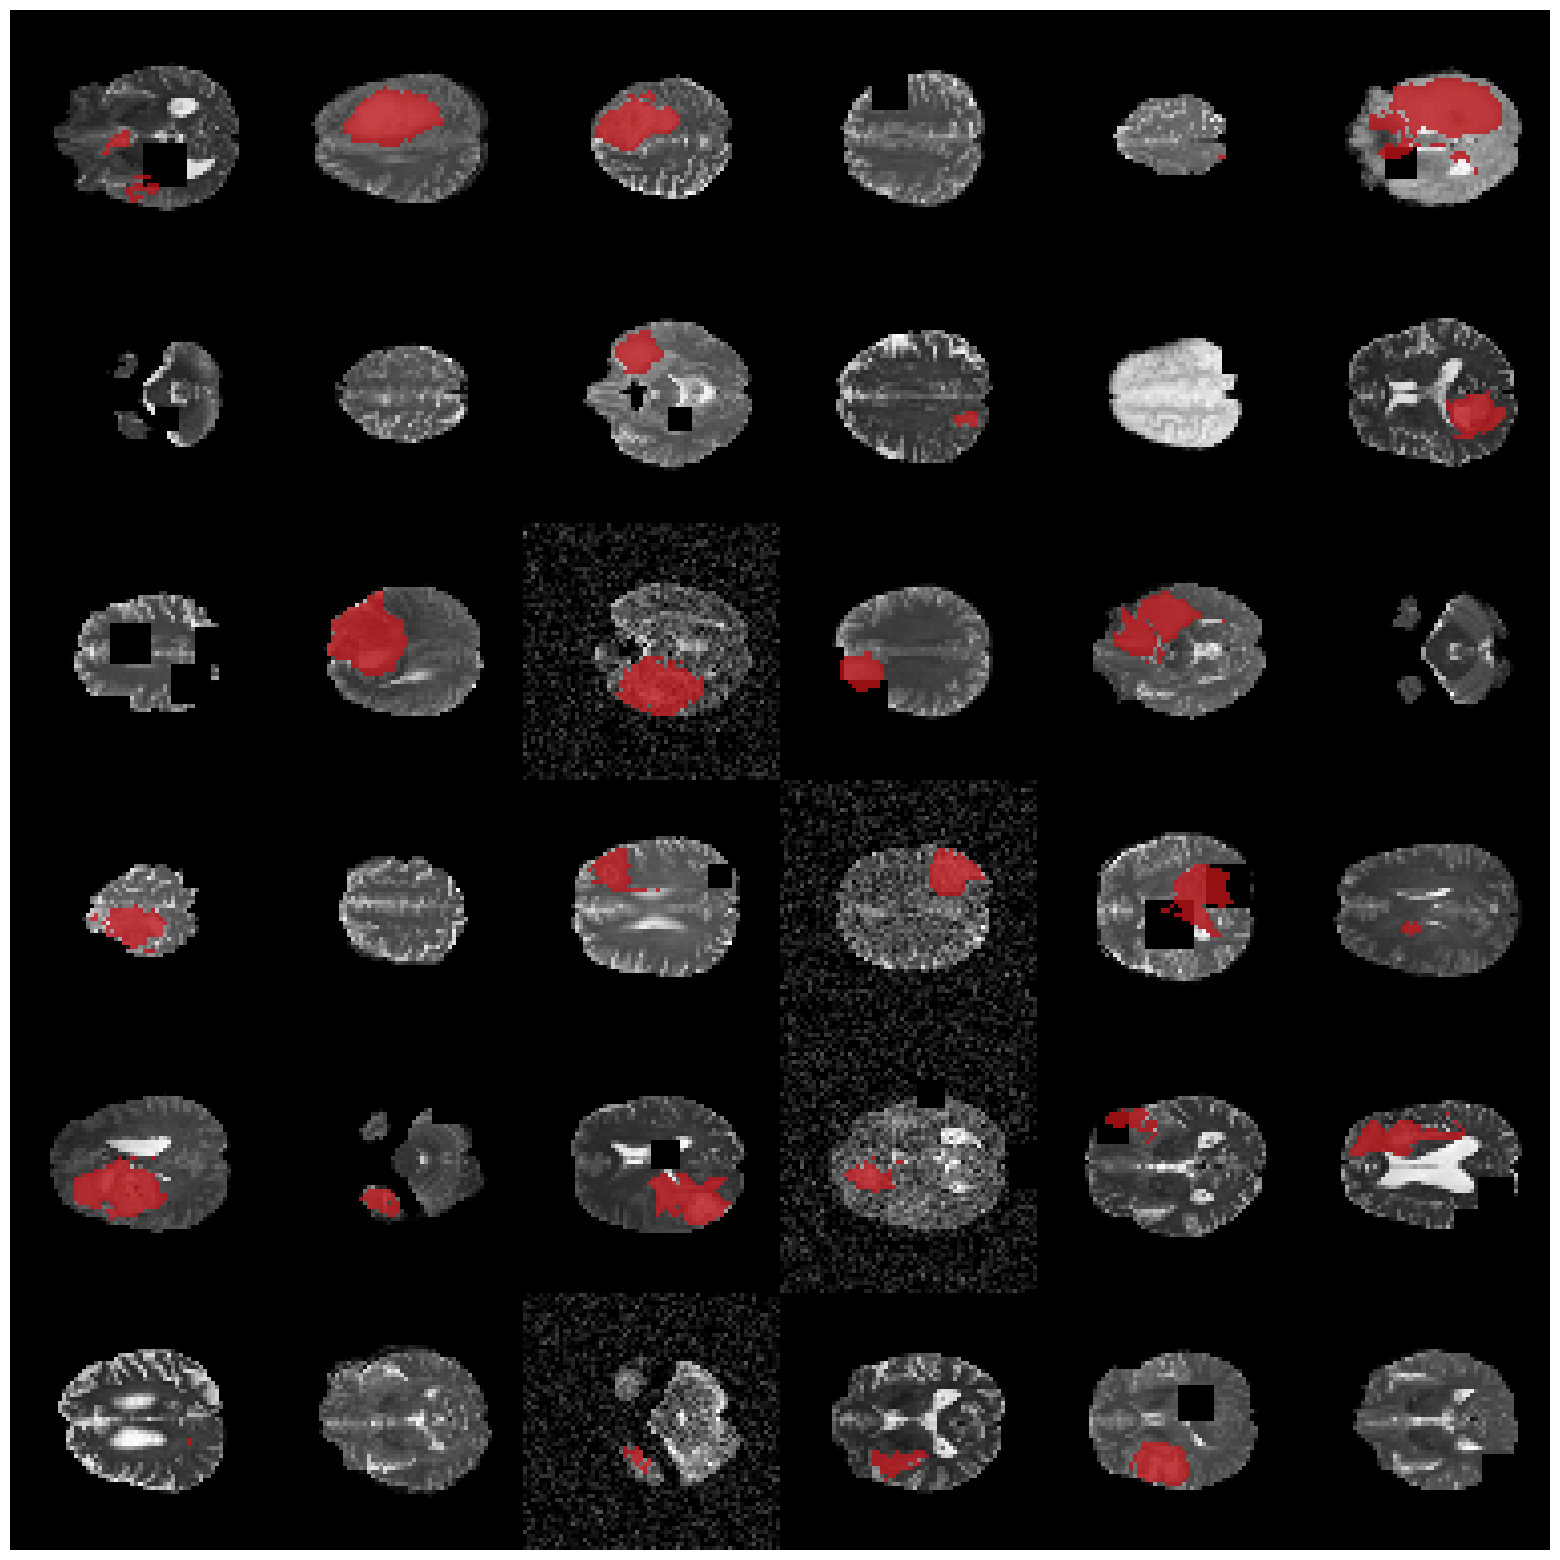
\includegraphics[width=0.9\textwidth]{report/Images/train_samples.png}
    \caption{Input samples to the model after pre-processing with augmentations. The shown channel is the one containing the FLAIR channel.}
    \label{fig:input_samples}
\end{figure*}


\end{document}